%%%%%%%%%%%%%%%%%%%%%%%%%%%%%%%%%%%%%%%%%%%%%%%%%%%%%%%%%%%%%%%%%%%%%%%%%%%%%%%%
%2345678901234567890123456789012345678901234567890123456789012345678901234567890
%        1         2         3         4         5         6         7         8
\documentclass[conference]{IEEEtran}
%\documentclass[letterpaper, 10 pt, conference]{ieeeconf}  % Comment this line out
                                                          % if you need a4paper
%\documentclass[a4paper, 10pt, conference]{ieeeconf}      % Use this line for a4
                                                          % paper

\IEEEoverridecommandlockouts                              % This command is only
                                                          % needed if you want to
                                                          % use the \thanks command
\overrideIEEEmargins
% See the \addtolength command later in the file to balance the column lengths
% on the last page of the document

\usepackage[utf8]{inputenc}
\usepackage[T1]{fontenc}
\usepackage[clean]{svg}
\usepackage{graphicx}
% The following packages can be found on http:\\www.ctan.org
%\usepackage{graphics} % for pdf, bitmapped graphics files
%\usepackage{epsfig} % for postscript graphics files
%\usepackage{mathptmx} % assumes new font selection scheme installed
%\usepackage{mathptmx} % assumes new font selection scheme installed
%\usepackage{amsmath} % assumes amsmath package installed
%\usepackage{amssymb}  % assumes amsmath package installed

\title{
Scradles - Dokumentation der Softwarearchitektur
}

\author{\IEEEauthorblockN{Aaron Kreuzer}
\IEEEauthorblockA{
a.kreuzer@oth-aw.de}
\and
\IEEEauthorblockN{Amos Asmerom}
\IEEEauthorblockA{
a.asmerom@oth-aw.de}
\and
\IEEEauthorblockN{Christoph Boni}
\IEEEauthorblockA{
c.boni@oth-aw.de}
\and
\IEEEauthorblockN{Leonard Wöllmer}
\IEEEauthorblockA{
l.woellmer@oth-aw.de}
\and
\IEEEauthorblockN{ Adrian Rall}
\IEEEauthorblockA{
a.rall@oth-aw.de}
\and
\IEEEauthorblockN{ Tahata Djoumsi}
\IEEEauthorblockA{
d.tahata@oth-aw.de}
}



\begin{document}



\maketitle
\thispagestyle{empty}
\pagestyle{empty}


%%%%%%%%%%%%%%%%%%%%%%%%%%%%%%%%%%%%%%%%%%%%%%%%%%%%%%%%%%%%%%%%%%%%%%%%%%%%%%%%
\begin{abstract}

Scradles ist eine online spielbare,
\\ crossplattformunabhängige Multiplayerversion von "Schere-Stein-Papier". Mehrere Spieler sollen dabei simultan, nicht rundenbasiert, mit der Plattform interagieren und gegeneinander antreten können. Eine Registrierung ist für den Nutzer optional; diese wird nur für den Eintrag in die globale Rangliste benötigt.

\end{abstract}


%%%%%%%%%%%%%%%%%%%%%%%%%%%%%%%%%%%%%%%%%%%%%%%%%%%%%%%%%%%%%%%%%%%%%%%%%%%%%%%%
\section{Mission Statement}
Onlinespiele wirken sich umso realer und realistischer auf die User Experience aus, wenn die Simultanität bei Interaktionen gegeben ist. Rundenbasierte Spiele können für taktische Spiele Übersicht und Kontinuität geben, für ein Gefühl realer Interaktivität ist diese Spielart im Onlinebereich aufgrund der entspehenden zeitlichen Verzögerungen jedoch unzureichend. Simultanität versprüht den Hauch von Nähe und realer Verständigung und Verbundenheit. Der Faktor Zeit spielt somit keine Rolle mehr, allein durch die räumliche Distanz unterscheiden sich  simultan gespielte Onlinespiele von "real life"-Interaktionen.
Ziel dieser Anwendung ist, Nutzern dieser Anwendung die Möglichkeit zu bieten, sich mit anderen Spielern online in Verbindung zu setzen und ihnen eine Plattform zu bieten, simultan und ohne erkennbare zeitlichen Interaktionsdifferenzen miteinander ein bereicherndes Erlebnis zu erschaffen.


%Sollte eig. die Graphik einbinden
\section{Kontextabgrenzung}

\begin{figure}[htbp]
\centering
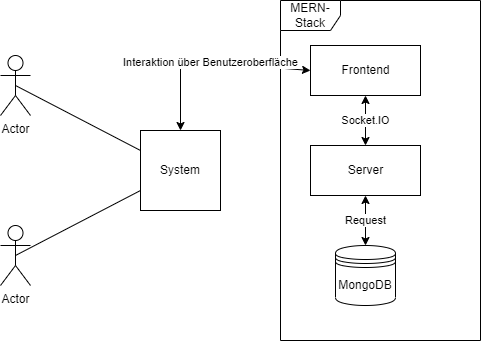
\includegraphics[scale=0.35]{Kontextabgrenzung.png}
\caption{Kontextabgrenzung}%
\end{figure}
\begin{itemize}


\subsection{Rahmenbedingungen}

Es wurde als Grundstruktur der MERN-Stack Framework verwendet.
Dieses Framework erleichtert es, eine 3-Schichten-Architektur aufzubauen. Dabei ist "MERN" ein Akronym für die darin verbauten Technologien:
\\
\begin{itemize}
    \item \textbf {M}ongoDB
    \item \textbf {E}xpressJS
    \item \textbf {R}eact
    \item \textbf {N}ode.js
\end{itemize}

MongoDB wird als grundlegende Datenbank verwendet. Darin können registrierte Spieler gespeichert werden und darauf basierend eine Bestenliste mit Punktestand generiert werden.
MongoDB gehört zu den sog. dokumentenbasierten NoSQL-Datenbanken. Ein großer Vorteil dieser Art von Abspeicherung und Strukturierung ist die einfache Verteilung der Arbeitslast auf mehrere Server.
\\
Express (manchmal auch als Express.js bezeichnet) ist ein Back-End-Webanwendungsframework, das auf Node.js ausgeführt wird.
\\
Node.js ist eine JavaScript-Laufzeitumgebung und ermöglicht die Implementierung von Javascript auf einem Server. Somit ist man in der Lage, einfach und unkompliziert Javascript außerhalb eines Browsers auszuführen und mit Datenbanken wie MongoDB zu verbinden.

\\
React ist eine JavaScript-Bibliothek, geeignet für das Erstellen von Web-Benutzeroberflächen. Ein großer Vorteil liegt in der Generierung wiedervewendbarer Komponenten, die auf jeweiligen Webseiten eingebunden werden können.
Für die Kommunikation zwischen den Schichten - Frontend und Server - also der Client-Server-Kommunikation, wird unter anderem Socket.IO verwendet. Diese Technologie erlaubt eine niedrige Latenzzeit und ermöglicht eine Skalierung auf mehrere Server und Senden von Ereignissen an alle verbundenen Clients.
\\
Desweiteren wird "nginx" verwendet, eine Webserver-Software zur Lastverteilung (umfangreiche Anfragen an einen Serversystem), um die aufkommenden Anfragen  auf mehrere Server zu verteilen. Dies hat eine effizientere Gesamtperformance zur Folge.
\\
Es wird Socket.IO für die Kommunikation zwischen Server und Clients genutzt. Socket.IO ist ebenfalls eine JavaScript-Bibliothek mit großen Stärken in der Echtzeit-Webanwendungsnutzung aufgrund seiner bidirektionalen Signalübertragung.

\section{Qualitätsziele}

Es gibt eine Liste an Qualitätszielen, welche erreicht werden soll.


\begin{itemize}
    \item Zuverlässigkeit \\
     \begin{itemize}
    \item  Das System soll immer in einem definierten Zustand verweilen.
    \item Jeder Link soll dabei zu einer weiteren Webseite führen.
    \item Alle Interaktionsartefakte (z.B. Buttons) sollen eine Funktionalität erfüllen. Interaktionsartefakte oder Verlinkungen ohne Funktion sind nicht vorgesehen.
    \item Damit wird verhindert, dass das System in einen undefinierten Zustand gerät und es zu einen Absturz der Anwendung kommt.
  \end{itemize}

    \item Funktionalität \\
    \begin{itemize}
        \item System soll zwei Clients verbinden können, sodass diese simultan an einen Spiel teilnehmen können.
        \item Das System soll die Spiellogik von "Schere-Stein-Papier" anwenden können.
        \item  Das System soll den Nutzern Rückmeldung über den Spielstand geben.
    \end{itemize}
    \item Benutzbarkeit \\
    \begin{itemize}
        \item Durch einen minimalistischen Aufbau werden die Interaktionsmöglichkeiten mit der Oberfläche auf das Nötige beschränkt.
        \item Dadurch wird das System schnell erlernbar und die Oberfläche erscheint intuitiv.
    \end{itemize}
    \item Sicherheit \\
    \begin{itemize}
        \item Nutzern wird nur eine geringe Interaktionsmöglichkeit geboten. Dies soll einen ausreichenden Zugriffs- und Veränderungsschutz von Daten ermöglichen.
    \end{itemize}

\end{itemize}
.

\section{Übersichtsbild}


%Bild MERN.png

\begin{figure}[htbp]
\centering
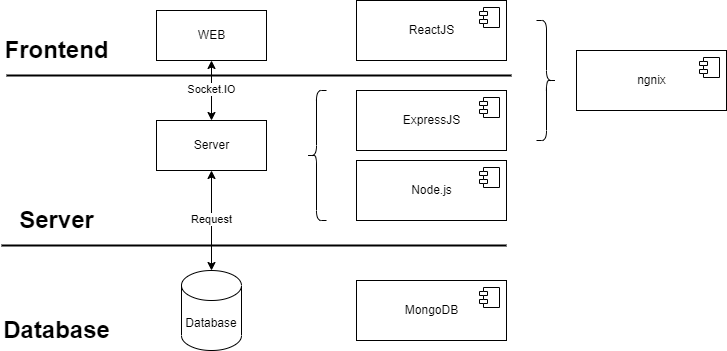
\includegraphics[scale=0.35]{MERN.png}
\caption{MERN-Stack-Schichtenmodell}%
\end{figure}
\begin{itemize}
Das 3-Schichten-Archtitekturmodell sieht eine Untergliederung in Benutzeroberfläche (Web-Frontend), Applikation (Server) und Datenbanksystem (Backend) vor. Dabei werden wie bereits erwähnt, die Javascript-Bibliothek "React" für das Frontend, die Technologien "ExpressJS" und "Node.js" für die serverseitige Logikebene verwendet. Als Datenbank kommt MongoDB zum Einsatz.
\\
Für die bidirektionale Kommunikation zwischen Client und Server wird Socket.IO verwendet.
\\
Desweiteren wird "nginx" für die Serverlastverteilung mit eingebunden. Nginx erlaubt durch seinen asynchronen Ansatz zur Verbindung mehrerer Request eine effizientere und geringe Speichernutzung und erhöht somit die Parallelisierung von Anfragen (Requests).

Mithilfe der Docker-Software können alle benötigten  Bibliotheken für alle Programmierer einheitlich und aktuell gehalten werden. Diese können dank der Software bereitgestellt und leicht verwaltet werden.

\end{itemize}

\section{Lösungsstrategie}

\begin{table}
\centering
\begin{tabular}{|l|l|ll}
\cline{1-2}
Effiziente und \\gute Antwortzeiten  & \begin{tabular}[c]{@{}l@{}}Mittels Lastverteilung durch nginx \\und Node.js sowie \\ durch ihre Eigenschaften der guten \\Skalierbarkeit von \\ Node.js und Socket.IO ~\end{tabular} &  &   \\
\cline{1-2}
Zuverlässigkeit und Funktionalität  & \begin{tabular}[c]{@{}l@{}} Es wurden sich an verschiedene \\
Programmierparadigmen gehalten und versucht,\\ anzuwenden. \\
Darunter: \\
- "Separation of Concerns", \\
- "Single Responsibility Principle" \\
- "Don't repeat yourself" und \\
- "Verständlichkeit"
~\end{tabular}                                     &  &   \\
\cline{1-2}
Benutzbarkeit   & \begin{tabular}[c]{@{}l@{}}Die 10 Heuristiken nach Jakob Nielsen \cite{c4} \\ für ein nutzbares User Interface \\ Design sind in die Anordnung \\ und Strukturierung \\ eingebracht worden.~\\ Ebenso ist die Norm \\ISO 9241-110 "Dialog \cite{c5}\\ principles" mitbedacht worden.\end{tabular}                                                      &  &   \\
\cline{1-2}
Sicherheit      & \begin{tabular}[c]{@{}l@{}}

Es werden neben der geringen \\ Eingabe- und Interaktionsmöglichkeit \\ keine weiteren sicherheitsrelevanten \\ (Verschlüsselungs-)Techniken eingesetzt ~\end{tabular}                                                                  &  &   \\
\cline{1-2}
\end{tabular}
\end{table}

\section{ARCHITEKTURPRINZIPIEN}
\subsection{Architekturprinzipien Frontend}
\begin{itemize}
    \item Modularität durch Components \\
    ("Separation of Concerns" +  \\
    \item Verständlichkeit des Codes \\
    ("DRY" + "KISS")
\end{itemize}
    \\Bei "DRY" (engl. für "Don't repeat yourself") ist ein Prinzip für eine gut strukturierte und verständliche Codekonvention. Ziel dieses Prinzips ist die Verminderung von Coderedundanz; also Vermeidung von Codereplikationen. Module sollen dabei einmal definiert und an geeigneter Stelle eingesetzt werden. Dies hat den Vorteil, dass Änderungen am Code nur einmal vorgenommen werden müssen und hat somit eine bessere Modularität zur Folge.
    \\Dieses Prinzip geht Hand-in-Hand mit dem Prinzip "KISS" (engl. "Keep it short, simple", deutsch: "Halte es kurz und simpel"). Dieses Apronym beschreibt die Idee, Code möglichst auf seine wesentlichen Aufgaben zu reduzieren. In Kombination mit dem DRY-Prinzip bedeutet dies, eine Funktion oder ein Modul mit lediglich einer Aufgabe zu definieren und mehrere Module, wenn nötig, ineinander zu verbauen.
    \\
    Das Prinzip "Seperation of Concerns" findet im Bereich der Programmiersprachenaufteilung statt. Es wird JavaScript für Funktions- und Moduldefinitionen genutzt, die äußere Erscheinung wird jedoch mittels CSS bearbeitet. (vgl. Wikipedia, 2022 \cite{c8})

\subsection{Architekturprinzipien Applikationsebene}
\begin{itemize}
    \item
    \item
    \item
    \item
\end{itemize}
\subsection{Architekturprinzipien Backend}
%Hier steht noch weiters zum Aufbau
%der Aufbau ist ab jetzt variabel, je nachdem, wo man 5voher schon etwas mit dazu geschrieben hat oder noch 5weiter erläutern möchte

\begin{itemize}
    \item \textbf {M}ongoDB
    \item \textbf {E}xpressJS
    \item \textbf {R}eactJS
    \item \textbf {N}ode.js
\end{itemize}



\section{MVP - MINIMUM VIABLE PRODUCT}
Das "Minimum viable product", kurz MVP, sieht vor, dass zwei Spieler gegeneinander in Echtzeit gegeneinander antreten können. Dabei soll jeder Spieler sich für eine von drei nutzbaren Antrittszustände wählen können (Schere, Stein oder Papier). Je nach Wahl des Artefaktes soll der Spielstand für die Nutzer ausgegeben werden. Es können mehrere Runden gegeneinander gespielt werden.
Nach einer gewissen Inaktivität, soll automatisch eine Beendigung des Spieles inkraft treten.
Ist ein Spieler registriert und angemeldet, wird die Anzahl seiner gewonnen Spiele in einer globalen Rangliste vermerkt. Es ist ein Spiel ohne Anmeldung oder Registrierung möglich.

\begin{figure}[htbp]
\centering
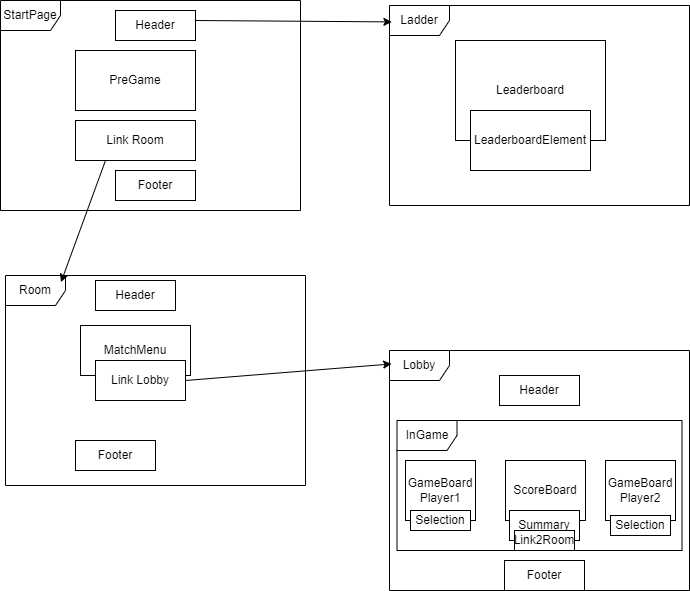
\includegraphics[scale=0.35]{FrontEndApplication.png}
\caption{Abbildung FrontEnd}%
\end{figure}
\begin{itemize}

\section{CONCLUSION}

\addtolength{\textheight}{-12cm}   % This command serves to balance the column lengths
                                  % on the last page of the document manually. It shortens
                                  % the textheight of the last page by a suitable amount.
                                  % This command does not take effect until the next page
                                  % so it should come on the page before the last. Make
                                  % sure that you do not shorten the textheight too much.

%%%%%%%%%%%%%%%%%%%%%%%%%%%%%%%%%%%%%%%%%%%%%%%%%%%%%%%%%%%%%%%%%%%%%%%%%%%%%%%%



%%%%%%%%%%%%%%%%%%%%%%%%%%%%%%%%%%%%%%%%%%%%%%%%%%%%%%%%%%%%%%%%%%%%%%%%%%%%%%%%



%%%%%%%%%%%%%%%%%%%%%%%%%%%%%%%%%%%%%%%%%%%%%%%%%%%%%%%%%%%%%%%%%%%%%%%%%%%%%%%%
\section*{APPENDIX}

Appendixes should appear before the acknowledgment.



%%%%%%%%%%%%%%%%%%%%%%%%%%%%%%%%%%%%%%%%%%%%%%%%%%%%%%%%%%%%%%%%%%%%%%%%%%%%%%%%

References are important to the reader; therefore, each citation must be complete and correct. If at all possible, references should be commonly available publications.



\begin{thebibliography}{99}
\bibitem{c4} Nielsen, Jakob. "usability heuristics. Nielsen Norman Group." (10).
\bibitem{c5} DIN, ENISO. Ergonomie der Mensch-System-Interaktion–Teil 110: Grundsätze der Dialoggestaltung (ISO 9241-110: 2006)[Ergonomics of human-system interaction–Part 110: Principles of dialogue design]. Deutsche Fassung EN ISO, S. 9241-110, 2006.
\bibitem{c6} S. Zörner.(2019, Dezember 09). Architektur ohne Firlefanz – Ihre Lösung auf einem Bierdeckel [online] Available: https://www.informatik-aktuell.de/entwicklung/methoden/architektur-ohne-firlefanz-ihre-loesung-auf-einem-bierdeckel.html
\bibitem{c6} MEHRA, Monika, et al. MERN stack Web Development. Annals of the Romanian Society for Cell Biology, 25. Jg., Nr. 6, S. 11756-11761, 2021.
\bibitem{c8} Wikipedia.(2022, Juni 17). Separation of concerns [online]
Available: https://en.wikipedia.org/wiki/Separation_of_concerns
\end{thebibliography}




\end{document}
